In this chapter we examine the structure of the consensus node: we see the
structure of the node and its main components, then, we show some snippets of code
in order to make clear the exact algorithm used.

As shown in the general architecture, %%TODO reference
the consensus node developed as a ROS node which subscribes and publishes messages
to different topics.
Moreover, the node offers some ROS services used to start and stop the trajectory
following algorithm or the consensus one.

The structure of the node takes into account the main architectural patterns used
in the software development field and it was designed to allow the maximum degree
of usability and customization, even though one of the most important metric taken
into account is the efficiency of the code, because of it has to be executed on
machines with limited amount of resources.

First of all, the node functionalities are enclosed into a C++ class which initializes
all the ROS elements and prepares the node to receive the start and stop commands.
The initialization is done by the class constructor when the object is created.
First of all, in order to apply the consensus dynamic equation, we need
the current position of the UAV. The Px4 publishes the estimated local position on
a topic, %%TODO reference
so, we need to subscribe to that topic to retrieve the messages with the needed
information.
Second, we want to publish the consensus variable of the drone in one topic used
by all the others, because, having obtained the others' consensus variables
from the same topic, we are able to compute the proportional consensus error.
Third, we need the next set point and the next desired velocity profile,
because we want to compute the error in position and weight it for the target velocity. %%TODO ref
At the end, we compute the acceleration of the consensus parameter using the consensus equation %%TODO ref
and we publish the next set point. We will see the details through the code.
All these elements can be summarized and shown in figure \ref{fig:node_in_out}.

\begin{figure}[h]
\centering
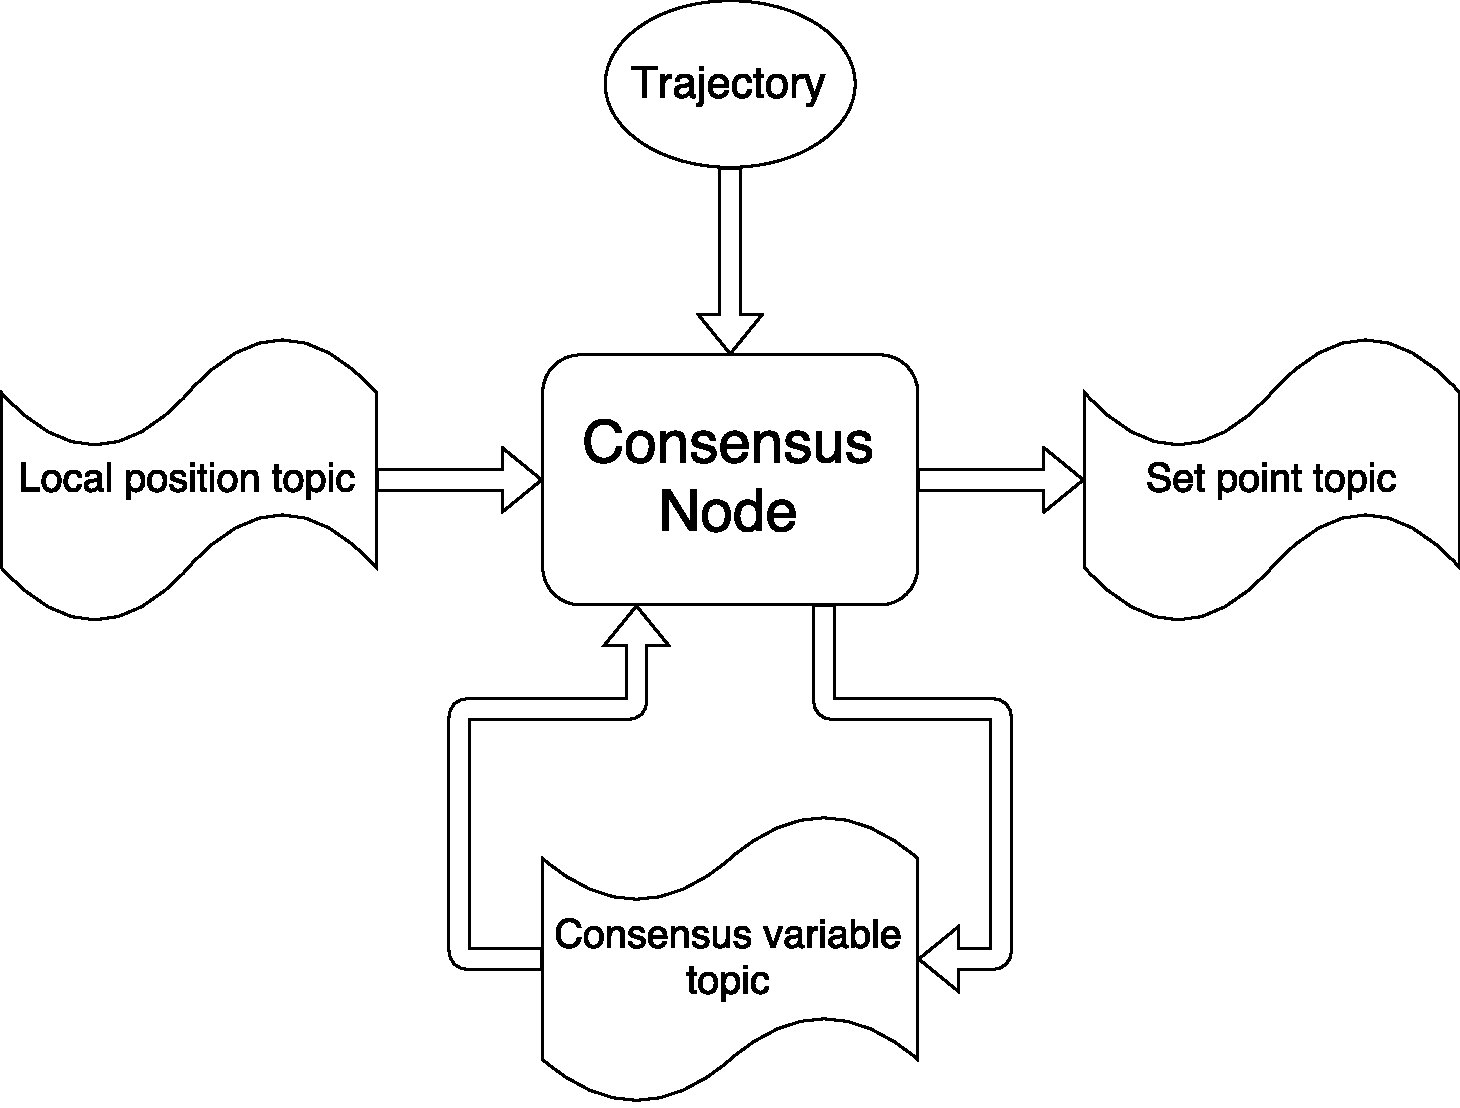
\includegraphics[width=0.9\textwidth]{chapters/chapter-04/figures/consensus_node_structure.pdf}
\caption{Input and output of the node}
\label{fig:node_in_out}
\end{figure}

The subscription of a ROS topic works with a callback function, which accepts as
parameter the pointer to the message. Since in our case we have multiple subscriptions
and we must advertise the start and stop services, we need to implement a multithreading
architecture which takes care of the concurrent accesses to the state of our object.
The number of thread used is three and these are their functions:
\begin{itemize}
  \item Start and stop services
  \item Consensus variable callback
  \item Local position callback
\end{itemize}

%% Sections of the chapter
\section{Start and stop services\label{sec:start_stop_services}}

First of all, the node can work in two different modes:
\begin{itemize}
  \item trajectory-only
  \item consensus
\end{itemize}

In the trajectory-only mode, the node computes the next set point and sends it to
the UAV, without taking care if there are others UAVs in the mission. Its only objective
is to follow the trajectory and reach its final position trying to respect the time
constraints imposed by the trajectory.
Instead, in the consensus mode, the node does the same computation as before, but
it also publishes its consensus variable and reads all the other ones.
It then considers this information and adjusts its variable.
The consensus mode includes the trajectory-only, and can be started even if the
trajectory-only is already started, while the opposite is not true. When you stop
the consensus mode, also the trajectory-only is stopped.
When the mission is accomplished, the current active mode is stopped automatically,
so that you can freely restart one of the two modes without the need of stopping
the previous one.

The services are implemented using the ROS Service class which manages the whole
infrastructure needed for calling the service. The call to the service is
synchronous and the caller is blocked until the service function is terminated.
In this case, we offer two services: one for starting and stoping the trajectory-only
mode and the other for the consensus mode.
It is possible to customize the service call in order to pass different number
and types of arguments to the service function and the response can also be
defined.
For the two services we have defined the same parameters that are shown in the figure
\ref{fig:custom_service}.

\begin{figure}[h]
\centering
  \lstinputlisting{chapters/chapter-04/code/FlyartCommandBool.srv}
\caption{Custom service structure}
\label{fig:custom_service}
\end{figure}

The message is composed by two parts: the request and the response.
In the request we need a boolean field in order to know if
we want to start or stop the algorithm. The response consists in a boolean variable
which represents the success of the operation and an exit code which identifies
the eventual problems occurred. The constants for the exit codes are directly specified
in the definition of the service.

The trajectory-only service starts or stops the thread which, taken a local position,
computes the next set point; while the consensus one starts or stops the same
thread as before and the one which retrieves the consensus variables from the other
quadrotors.


\input{chapters/chapter-04/consensus_variable_loopback.tex}

\input{chapters/chapter-04/local_position_loopback.tex}
